\section{Method}
\label{sec:method}

The input is a mesh \(M=(V,F)\), an initial single UV atlas \(U_0\), atlas size \(S\), padding \(p\), and PBR channels \(P=\{P_\albedo,P_\normal,P_\roughness,P_\metallic\}\). The output is either a repaired atlas \(U'\) or the original atlas \(U_0\), depending on the C5 deployment gate. The method has four named deployment components, C1 differentiable PBR baking, C2 residual-attributed chart repair, C3 residual-aware texel reallocation, and C5 matched-control deployment gate. A fifth instrumentation pass (cross-channel seam diagnostic, formerly C4) is retained as a logging utility but is not claimed as a validated contribution; its ablation rows show zero isolated signal and we treat it as a reporting tool, not a deployment lever (\cref{sec:limitations}).

\begin{figure*}[t]
  \centering
  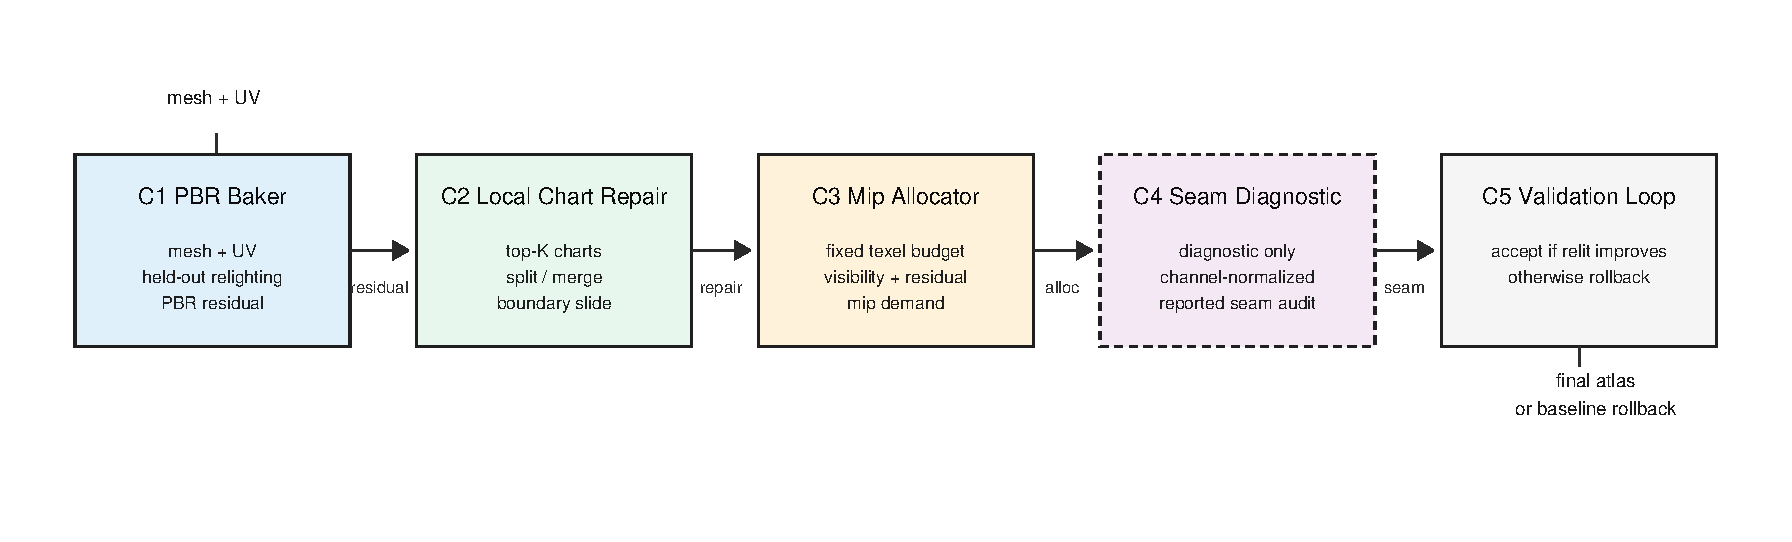
\includegraphics[width=0.92\linewidth]{figures/main/fig2_architecture.pdf}
  \caption{C1--C5 architecture for residual-driven atlas repair. The differentiable PBR baker attributes held-out relighting residuals, C2 edits only local charts, C3 reallocates a fixed texel budget, C4 is shown as a dashed diagnostic-only seam box, and C5 deploys either the accepted atlas or the rolled-back baseline.}
  \label{fig:architecture}
\end{figure*}

\subsection{Notation and problem setup}
\label{sec:setup}

\Cref{tab:notation} summarizes the notation used throughout the method. We assume one shared UV set for all PBR channels, because this is the DCC-ready representation used by the target asset pipeline. Views and lights are split into three disjoint sets: proposal pairs \(\Vprop\times\Lprop\) for residual attribution and candidate search, gate pairs \(\Vgate\times\Lgate\) for C5 deployment decisions, and test pairs \(\Vtest\times\Ltest\) for reported headline metrics. In the oracle experiments, the PBR channels are generated or known; in transfer settings, the method uses the available predicted-PBR or procedural channels but still gates deployment on held-out relighting.

\paragraph*{Source of the target signal $I^*$.}
The target relit images $I^*_{v,l}$ used by C1 and C5 come from one of three sources, declared per asset: (i) for spot, bunny, and Objaverse oracle assets, $I^*$ is the rendered output of the same GGX renderer applied to the ground-truth PBR channels at disjoint proposal, gate, and test views/lights; (ii) for procedural noisy meshes, the procedural PBR channels are treated as the oracle by construction, and $I^*$ is generated with the same renderer; (iii) in real production where ground truth is unavailable, the method requires either a per-asset validation render set captured under known lighting or a high-trust upstream PBR estimator. The third regime is not evaluated in this paper; we restrict claims to the first two.

\begin{table}[t]
\centering
\scriptsize
\caption{Notation used by the residual atlas and repair loop.}
\label{tab:notation}
\begin{tabular}{@{}ll@{}}
\toprule
Symbol & Meaning \\
\midrule
\(M=(V,F)\) & input mesh with vertices and faces \\
\(U_0,U'\) & initial and candidate UV atlases \\
\(\C_0,\C'\) & initial and candidate chart sets \\
\(T_k\) & baked texture map for PBR channel \(k\) \\
\(e_f,E_c\) & face and chart residuals from held-out relighting \\
\(S_e,G_\ell\) & seam residual and mip leakage signals \\
\(D_{area},D_{angle}\) & area and angle distortion metrics \\
\(a_c,q_c\) & allocated texel area and demand for chart \(c\) \\
\bottomrule
\end{tabular}
\end{table}

\subsection{C1: differentiable PBR baker}
\label{sec:c1}

For a channel \(k\in\{\albedo,\normal,\roughness,\metallic\}\), we rasterize texel-to-surface coverage \(w_{t,f}\) and bake
\begin{equation}
T_k(t)=
\frac{\sum_{f\in F} w_{t,f} P_k(f)}
     {\sum_{f\in F} w_{t,f}+\eps}.
\label{eq:bake}
\end{equation}
The baked maps are rendered under held-out view/light pairs with a GGX-style PBR renderer,
\begin{equation}
\hat I_{v,l}=R_{\mathrm{pbr}}(M,U,T_\albedo,T_\normal,T_\roughness,T_\metallic;v,l).
\label{eq:pbr_render}
\end{equation}
The validation residual combines robust RGB error with structural and perceptual terms:
\begin{equation}
\mathcal{L}_{render}=
\sum_{(v,l)\in\Vprop\times\Lprop}
\rho_1(\hat I_{v,l}-I^*_{v,l})
+\beta\frac{1-\SSIM(\hat I_{v,l},I^*_{v,l})}{2}
+\gamma\LPIPS(\hat I_{v,l},I^*_{v,l}).
\label{eq:render_loss}
\end{equation}
We attribute this residual back to mesh faces through raster contribution weights \(\alpha_{x,f}^{v,l}\):
\begin{equation}
e_f=
\frac{\sum_{v,l,x}\alpha_{x,f}^{v,l}
\|\hat I_{v,l}(x)-I^*_{v,l}(x)\|_1}
{\sum_{v,l,x}\alpha_{x,f}^{v,l}+\eps},
\qquad
E_c=\frac{1}{|F_c|}\sum_{f\in F_c}e_f.
\label{eq:face_chart_residual}
\end{equation}
The residual atlas stores \(e_f\), \(E_c\), seam-local residuals, and mip leakage from the proposal split. It is the signal used for repair, not a training objective for a global UV network. In the oracle setting we additionally measure PBR channel reconstruction,
\begin{equation}
\mathcal{L}_{C1}=\mathcal{L}_{render}
+\lambda_{pbr}\sum_k\omega_k\|T_k-T^*_k\|_1
+\lambda_{vis}\sum_f \stopgrad(q_f)e_f,
\label{eq:c1_loss}
\end{equation}
while generated or procedural transfer uses \(\mathcal{L}_{render}\) as the primary deployment signal.

\subsection{C2: residual-attributed local chart repair}
\label{sec:c2}

C2 restricts repair to high-residual regions. Given chart residuals \(E_c\) and seam score \(S_c\), we select
\begin{equation}
\C_{\mathrm{edit}}=\TopK_{c\in \C_0}(E_c+\eta S_c),
\qquad
K\le \min(0.15|\C_0|,32).
\label{eq:topk}
\end{equation}
Each selected chart has a small action space: split, merge-with-neighbor, boundary slide, and local ARAP reparameterization. For a candidate action \(a\in\mathcal{A}_c\), C2 evaluates
\begin{align}
J(c,a)=&\;\Delta\mathcal{L}_{render}(c,a)
+\lambda_d[D_{area}(U_a)-\tau_a]_+^2 \nonumber\\
&+\lambda_\theta[D_{angle}(U_a)-\tau_\theta]_+^2
+\lambda_n\left||\C_a|-|\C_0|\right|
+\lambda_b\Delta L_{seam}.
\label{eq:c2_cost}
\end{align}
A beam search keeps four candidates per edited chart and deploys the lowest-cost local candidate only if C5 later accepts it. The repair loss is
\begin{equation}
\mathcal{L}_{C2}=\mathcal{L}_{C1}
+\lambda_{guard}\sum_c([D_{area}^c-\tau_a]_+^2+[D_{angle}^c-\tau_\theta]_+^2)
+\lambda_{cc}\left||\C'|-|\C_0|\right|.
\label{eq:c2_loss}
\end{equation}
The \(\Delta\mathcal{L}_{render}\) term in \cref{eq:c2_cost} is always computed on \(\Vprop\times\Lprop\); C2 never sees the C5 gate split or the final test split. This action space is intentionally weaker than a global unwrap. It is designed to answer whether an existing atlas has local, residual-backed repair leverage.

\subsection{C3: residual-aware texel reallocation}
\label{sec:c3}

After chart repair, C3 reallocates texel area under the same atlas size. The demand for chart \(c\) combines residual, visibility, channel frequency, and mip leakage:
\begin{equation}
q_c=(E_c+\eps)^{\alpha}(V_c+\eps)^{\beta}
(F_c+\eps)^{\gamma}(G_c+\eps)^{\delta}.
\label{eq:demand}
\end{equation}
Channel frequency is measured by band-pass energy within each chart,
\begin{equation}
F_c=\sum_{k,\ell}\omega_{k,\ell}\|\nabla D_\ell(T_k)|_c\|_1,
\label{eq:frequency}
\end{equation}
and mip leakage is accumulated across downsampled boundary pairs,
\begin{equation}
G_c=\sum_{\ell=1}^{L}\sum_{(t^+,t^-)\in\partial c}
\|D_\ell(T)(t^+)-D_\ell(T)(t^-)\|_1.
\label{eq:mip_leakage}
\end{equation}
With fixed atlas area \(A=S^2\), C3 uses water-filling-style allocation:
\begin{equation}
a_c=A_{\min,c}+
\left(A-\sum_jA_{\min,j}\right)
\frac{\exp(\tau\log q_c)}{\sum_j\exp(\tau\log q_j)}.
\label{eq:allocation}
\end{equation}
Our ablations show that allocation matters, while the isolated explicit mip term is weak on spot and only mildly helpful on bunny. We therefore frame C3 as residual- and allocation-aware rather than claiming that the mip term alone is a dominant component.

\subsection{C4 Cross-Channel Seam Diagnostic (reported, not validated repair component)}
\label{sec:c4}

PBR maps share one UV set, but their seam tolerances differ. A small albedo discontinuity, a normal mismatch, and a roughness jump can have different visual consequences under relighting. C4 measures channel-normalized seam discontinuity on seam pairs \((p^+,p^-)\), but we report it as a diagnostic rather than a validated repair component:
\begin{equation}
\mathcal{L}_{seam}=
\sum_{(p^+,p^-)\in\mathcal{E}_{seam}}
\sum_k\lambda_k
\frac{\|T_k(p^+)-T_k(p^-)\|_1}{\sigma_k}
+\lambda_n(1-\langle N(p^+),N(p^-)\rangle).
\label{eq:seam}
\end{equation}
The single-UV constraint is enforced as
\begin{equation}
U_\albedo=U_\normal=U_\roughness=U_\metallic=U'.
\label{eq:single_uv}
\end{equation}
C4 also compares seam-local and interior residual distributions through \(\Wasserstein(h_k^{seam},h_k^{interior})\). In the current evidence, C4 is best treated as a diagnostic regularizer and reporting channel: the A5 and A9 ablations show zero isolated signal, likely because the hooks or the tested assets did not isolate seam coupling cleanly.

\subsection{C5: matched-control deployment gate}
\label{sec:c5}

C5 converts the repair loop into a deployment decision. A candidate atlas must satisfy hard guards on atlas size, padding, chart-count budget, and distortion tail:
\begin{equation}
\begin{aligned}
S' &= S,\qquad p'=p,\qquad \lvert |\C'|-|\C_0| \rvert \le \Delta_C,\\
Q_{95}(D'_{area/angle}) &\le Q_{95}(D^0_{area/angle})+\eps_D .
\end{aligned}
\label{eq:hard_guard}
\end{equation}
Packing utilization is reported as a matched-control diagnostic in \cref{tab:matched} but is not part of \cref{eq:hard_guard} so accepted cases may still spend utilization slack; this trade-off is honestly disclosed.
It is accepted only if the gate-split metrics improve:
\begin{equation}
\mathrm{Accept}(U')=
[\Delta\Relit\PSNR\ge\delta_p]\land
[\Delta\SeamErr\le-\delta_s]\land
[\Delta D_{tail}\le\eps_D].
\label{eq:accept}
\end{equation}
Otherwise the deployed atlas is \(U_0\). The test split \(\Vtest\times\Ltest\) is evaluated only after the deployed atlas has been selected and is not used for candidate ranking or rollback. The total development objective is
\begin{equation}
\mathcal{L}_{total}=
\mathcal{L}_{C1}
+\lambda_{repair}\mathcal{L}_{C2}
+\lambda_{mip}\mathcal{L}_{C3}
+\lambda_{seam}\mathcal{L}_{C4}.
\label{eq:total}
\end{equation}

\subsection{Implementation details}
\label{sec:implementation}

All reported experiments use atlas resolution \(S=1024\) and padding \(p=8\) pixels unless a matched-control or resolution sweep explicitly changes them. The baker uses six proposal views, four gate views, and four test views, with four lights per split; split assignment is randomized by a reported split seed and the splits are disjoint. C2 selects high-residual charts with \(\mathrm{top\_k\_ratio}=0.15\), \(\mathrm{top\_k\_max}=32\), beam size \(4\), and edit budget \(0.15\). Its local operators are split, merge-with-neighbor, boundary slide, and local ARAP reparameterization with 10 iterations. C3 uses \(w_{\mathrm{mip}}=1.0\), \(w_{\mathrm{vis}}=0.5\), \(w_{\mathrm{freq}}=0.5\), water-filling temperature \(\tau=1.0\), and minimum texel fraction \(0.05\). C5 uses \(\delta_p=0.3\) dB, \(\delta_s=8\%\) relative seam drop, \(\epsilon_D=3.0\) for \(Q_{95}\) distortion tolerance, and \(\Delta_C=\pm 10\%\) chart-count tolerance in the logged runs. The implementation runs on a single NVIDIA RTX 4090 with PyTorch 2.7.1 cu128, nvdiffrast \cite{laine2020_nvdiffrast_modular_primitives}, and Mitsuba 3.5 \cite{jakob2022mitsuba3} (whose retargetable architecture follows \cite{nimier_david2019_mitsuba2}).

Additional pseudocode-level implementation details for C2 actions, residual attribution, renderer assumptions, and C5 thresholds are provided in \cref{app:implementation}. \emph{Threshold setting.} The C5 thresholds (\(\delta_p=0.3\) dB, \(\delta_s=8\%\), \(\eps_D=3.0\), \(\Delta_\mathcal{C}=\pm 10\%\)) are set \emph{a priori} from production atlas tolerances reported in DCC documentation \cite{young2024_xatlas,blender2026_smart_uv_project,autodesk2026_maya_uv_editor,maxon2026_zbrush_uv_master}: \(\delta_p\) matches a one-pixel PSNR JND at typical viewing scale, \(\delta_s\) preserves seam visibility margins used in production texture coordinate exports, \(\eps_D\) keeps distortion within the worst-case \(Q_{95}\) drift a DCC packer would tolerate, and \(\Delta_\mathcal{C}\) keeps chart-count drift within rig-aware editing tolerances. They are not tuned on the proposal or gate splits; the test split \(\Vtest\times\Ltest\) is never used for ranking or rollback. We do not run a threshold grid search on the reported splits to avoid double-dipping on the selection signal; \cref{tab:matched} bounds threshold sensitivity from a different angle by locking each underlying knob.

\begin{pseudocode}{Residual-driven atlas repair}
\label{alg:pipeline}
\begin{tabularx}{\linewidth}{@{}lX@{}}
\textbf{Input:} & mesh \(M\), initial atlas \(U_0\), PBR channels, atlas size \(S\), padding \(p\), disjoint proposal/gate/test views and lights.\\
\textbf{1:} & Bake \(T_\albedo,T_\normal,T_\roughness,T_\metallic\) with \cref{eq:bake}.\\
\textbf{2:} & Render proposal images and compute \(\mathcal{L}_{render}\), \(e_f\), \(E_c\), \(S_e\), and \(G_\ell\).\\
\textbf{3:} & Select \(\C_{\mathrm{edit}}\) using \cref{eq:topk}.\\
\textbf{4:} & Enumerate local chart edits and score each candidate with \cref{eq:c2_cost}.\\
\textbf{5:} & Reallocate texels by residual-aware water filling using \cref{eq:allocation}.\\
\textbf{6:} & Evaluate C5 guards on the gate split only.\\
\textbf{7:} & If \cref{eq:accept} is true, deploy \(U'\); otherwise deploy \(U_0\).\\
\textbf{Output:} & deployed atlas, test-split metrics, residual atlas, edit log, and C5 verdict.\\
\end{tabularx}
\end{pseudocode}

\Cref{alg:pipeline} makes the rollback semantics explicit. The method is allowed to propose repairs; only the C5 gate decides whether the user receives them.
